\documentclass[14pt]{article}
\usepackage{amsmath}
\usepackage{amssymb}
\usepackage{cancel}
\usepackage{graphicx}
\usepackage{geometry}
\geometry{
	a4paper,
	total={170mm,257mm},
	left=20mm,
	bottom=20mm,
	top=0mm,
}
\begin{document}
	\title{Line Integral and Rotation Examples}
	\author{Saptarshi Dey}
	\maketitle
	\section{Line Integrals Examples}
	\subsection{Questions}
	\large{
		1. Evaluate $\displaystyle \int\limits_{C}{{3{x^2} - 2y \,ds}}$ where C is the line segment from $\left( {3,6} \right)$ to $\left( {1,-1} \right)$}
	\\ \large{
		2. Evaluate $\displaystyle \int\limits_{C}{{2y{x^2} - 4x\,ds}}$ where C is the lower half of the circle centered at the origin of radius 3 with clockwise rotation.}
	\\ \large{
		3. Evaluate $\displaystyle \int\limits_{C}{{6x\,ds}}$ where C is the portion of $y = {x^2}$ from $x=-1$ to $x=2$. The direction of C is in the direction of increasing x.}
	\\ \large{
		4. Evaluate $\displaystyle \int\limits_{C}{{xy - 4z\,ds}}$ where C is the line segment from $\left( {1,1,0} \right)$ to $\left( {2,3,-2} \right)$}
	\\ \large{
		5. Evaluate $\displaystyle \int\limits_{C}{{{x^2}{y^2}\,ds}}$ where C is the circle centered at the origin of radius 2 centered on the $y$-axis at $y=4$. See the sketches below for orientation.}
	\\ \begin{center}
		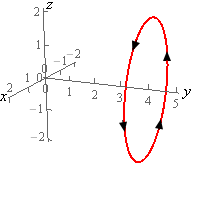
\includegraphics[width=0.35\textwidth]{"./Pictures/Q5_1.png"}
		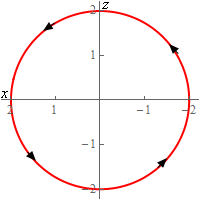
\includegraphics[width=0.35\textwidth]{"./Pictures/Q5_2.png"}
	\end{center}
	\large{
		6. Evaluate $\displaystyle \int\limits_{C}{{16{y^5}\,ds}}$ where C is the portion of $x=y^4$ from $y=0$ to $y=1$ followed by the line segment form $\left( {1,1} \right)$ to $\left( {1,-2} \right)$ which in turn is followed by the line segment from $\left( {1,-2} \right)$ to $\left( {2,0} \right)$. See the sketch below for the direction.
	}
	\\ \begin{center}
		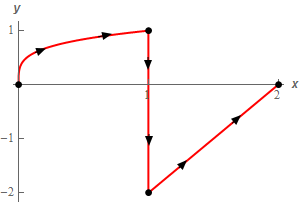
\includegraphics[width=0.35\textwidth]{"./Pictures/Q6.png"}
	\end{center}
	\bigskip \bigskip \bigskip
	\pagebreak
	\hspace{10pt}
	\subsection{Solutions}
	\large{
		1. Using the point-slope formula, we have $\displaystyle (y+1)=\frac{7}{2} (x-1)
		\\ \therefore 2y=7x-9 \implies 2 dy = 7 dx \implies \frac{dy}{dx}=\frac{7}{2}
		\\ \therefore ds=\sqrt{1+\left( \frac{dy}{dx}\right)^2}=\sqrt{1+\left( \frac{7}{2}\right)^2}=\frac{\sqrt{53}}{2}\,dx
		\\ \therefore \int\limits_{C}{{3{x^2} - 2y \,ds}}=\int\limits_{1}^{3} \left(3x^2-7x+9\right) \frac{\sqrt{53}}{2} \,dx=\frac{\sqrt{53}}{2} \left[x^3-\frac{7x^2}{2}+9x\right]_1^3=\boxed{8\sqrt{53}}$}
	\\ \\ \large{
		2. Let $x=3\cos{\theta}$ and $y=3\sin{\theta}$
		\\$ \displaystyle \therefore ds=\sqrt{\left(\frac{dx}{d\theta}\right)^2+\left(\frac{dy}{d\theta}\right)^2} d\theta=3\sqrt{\sin^2{\theta}+\cos^2{\theta}}d\theta=3\,d\theta
		\\ \therefore \int\limits_{C}{{2y{x^2} - 4x\,ds}}=3\int\limits_\pi^{2\pi} (54\sin\theta\cos^2\theta-12\cos\theta)\,d\theta=-162\int\limits_{-1}^{1} u^2 du+\cancel{12\left[\sin\theta\right]_\pi^{2\pi}}=\boxed{-108}$}
	\\ \\ \large{
		3. $\displaystyle y=x^2 \implies\frac{dy}{dx}=2x
		\\ \therefore ds=\sqrt{1+\left(\frac{dy}{dx}\right)^2}dx=\sqrt{1+4x^2}\,dx  
		\\ \therefore \int\limits_{C}{{6x\,ds}}=\int\limits_{-1}^2 6x\sqrt{1+4x^2}\,dx=\frac{3}{4}\int\limits_{5}^{17}{\sqrt{u}\,du}=\boxed{\frac{17^{1.5}-5^{1.5}}{2}}$}
	\\ \\ \large{
		4. First we have to calculate the direction cosines of the line.\\
		$\therefore \displaystyle l=1,m=2,n=-2$
		\\ $\therefore$ The required equation of the line is $\displaystyle \frac{x-1}{1}=\frac{y-1}{2}=\frac{z-0}{-2}$
		\\$\displaystyle \therefore z=-2x+2$ and $\displaystyle y=2x-1$
		\\ $\displaystyle \implies \frac{dz}{dx}=-2$ and $\displaystyle \frac{dy}{dx}=2
		\\ \therefore ds=\sqrt{1+\left(\frac{dy}{dx}\right)^2+\left(\frac{dz}{dx}\right)^2}dx=\sqrt{1+2^2+(-2)^2}dx=3dx
		\\ \therefore \int\limits_{C}{{xy - 4z\,ds}}=3\int\limits_1^2 x(2x-1)+8(x-1)dx=3\left[\dfrac{x\cdot\left(4x^2+21x-48\right)}{6}\right]_1^2=\boxed{\frac{43}{2}}$}
	\\ \\ \large{
		5. Let $x=2\cos\theta$ and $z=2\sin\theta$
		\\ $\displaystyle \therefore ds=\sqrt{\left(\frac{dx}{d\theta}\right)^2+\left(\frac{dz}{d\theta}\right)^2}=2\sqrt{\sin^2{\theta}+\cos^2{\theta}}d\theta=2d\theta
	\\ \therefore \int\limits_{C}{{{x^2}{y^2}\,ds}}=64\int\limits_0^{2\pi}2 \sin^2\theta d\theta=64\left(\int\limits_0^{2\pi}d\theta-\int\limits_0^{2\pi}\cos 2\theta d\theta\right)=128\pi-\cancel{32\left[\sin2\theta\right]_0^{2\pi}}=\boxed{128\pi}$}
	\\ \\ \large{
		6. $\displaystyle \int\limits_{C}{{16{y^5}\,ds}}=\int\limits_{C_1}{{16{y^5}\,ds}}+\int\limits_{C_2}{{16{y^5}\,ds}}+\int\limits_{C_3}{{16{y^5}\,ds}}
		\\ C_1\equiv x=y^4,\left[0\leq y\leq1\right],ds=\sqrt{1+(4y^3)^2}dy=\sqrt{1+16y^6}dy
		\\ C_2\equiv x=1,\left[-2\leq y\leq1\right],ds=\sqrt{1+0^2}dy=dy
		\\ C_3\equiv x=\frac{y}{2}+2,\left[-2\leq y\leq0\right],ds=\sqrt{1+\left(\frac{1}{2}\right)^2}dy=\frac{\sqrt{5}}{2}dy$}
	\pagebreak
	\hspace{10pt}
	\\ \\ \large{
		$\displaystyle \int\limits_{C}{{16{y^5}\,ds}}=\int\limits_{0}^{1}16y^5\sqrt{1+16y^6}\,dy+16\int\limits_{-2}^{1}y^5\,dy+8\sqrt{5}\int\limits_{-2}^{0}y^5\,dy
		\\ = \frac{1}{6}\int\limits_{1}^{17}\sqrt{u}\,du+\frac{8}{3}\left[y^6\right]_{-2}^1+\frac{4\sqrt{5}}{3}\left[y^6\right]_{-2}^0=\frac{1}{9}\left[u^{1.5}\right]_1^{17}-168-\frac{256\sqrt{5}}{3}
		\\=\frac{17^{1.5}-1}{9}-168-\frac{256\sqrt{5}}{3}=\boxed{-351.1341}$}
	\section{Rotation of Coordinate Systems}
	\subsection{Rotation Matrices}
	\large{
		The 2D Rotation Matrix is $\begin{bmatrix}
		\cos\theta & -\sin\theta\\
		\sin\theta & \cos\theta
		\end{bmatrix}$ where $\theta$ is the angle of rotation.
		\\ \\ The 3D Rotation Matrices are:-
		\\ \\ About X-Axis $R_x(\theta)$= $\displaystyle \begin{bmatrix}
		1 & 1 & 0\\
		0 & \cos\theta & -\sin\theta\\
		0 & \sin\theta & \cos\theta
		\end{bmatrix}$
		\\ \\ About Y-Axis $R_y(\theta)$= $\displaystyle \begin{bmatrix}
		\cos\theta & 0 & \sin\theta\\
		0 & 1 & 0\\
		-\sin\theta & 0 & \cos\theta
		\end{bmatrix}$
		\\ \\ About Z-Axis $R_z(\theta)$= $\displaystyle \begin{bmatrix}
		\cos\theta & -\sin\theta & 0\\
		\sin\theta & \cos\theta & 0\\
		0 & 0 & 1
		\end{bmatrix}$}
	\subsection{Example}
	\large{
		If the Axes are rotated through 60\textdegree $\,$ in the anticlockwise direction, find the transformed form of the equation $x^2-y^2=a^2$
	}
	\\ \\ \large{
		\textbf{Soln:-} Let the transformed coordinates be $X$ and $Y$.
		$\\ \\ \displaystyle \therefore \begin{bmatrix}
		x \\ y
		\end{bmatrix}=\begin{bmatrix}
			\cos60 & -\sin60\\
			\sin60 & \cos60
		\end{bmatrix}
		\begin{bmatrix}
		X \\ Y
		\end{bmatrix}
		=\frac{1}{2}\begin{bmatrix}
		X-\sqrt{3}Y \\ \sqrt{3}X+Y
		\end{bmatrix}$
		\\ \\ Putting the values of x and y in the given equation we get
		\\ $\displaystyle \left(X-\sqrt{3}Y\right)^2-\left(\sqrt{3}X+Y\right)^2=4a^2
		\\ \\ \implies 2Y^2-2X^2-4\sqrt{3}XY=4a^2 \implies \boxed{Y^2-X^2-2\sqrt{3}XY=2a^2}$
	}
\end{document}